\documentclass{beamer}
\usepackage{listings}
\usepackage{xcolor}
\usepackage{tikz}
\usetikzlibrary{decorations.pathreplacing, decorations.markings, patterns}
\usepackage{courier}
\usepackage[utf8]{inputenc}
\usepackage{textcomp}  % For micro symbol

\definecolor{codegreen}{rgb}{0,0.6,0}
\definecolor{codegray}{rgb}{0.5,0.5,0.5}
\definecolor{codepurple}{rgb}{0.58,0,0.82}
\definecolor{backcolour}{rgb}{0.95,0.95,0.95}

\lstdefinestyle{mystyle}{
    backgroundcolor=\color{backcolour},
    commentstyle=\color{codegreen},
    keywordstyle=\color{blue},
    stringstyle=\color{codepurple},
    basicstyle=\ttfamily\scriptsize,  % Smaller font size
    breakatwhitespace=false,
    breaklines=true,
    captionpos=b,
    keepspaces=true,
    numbersep=5pt,
    showspaces=false,
    showstringspaces=false,
    showtabs=false,
    tabsize=2
}

\lstset{style=mystyle}

\title{Lock-Free Ring Buffer for Market Data}
\author{Low Latency Data Pipeline Team}
\date{\today}

\begin{document}

\begin{frame}
\titlepage
\end{frame}

\begin{frame}{Outline}
\tableofcontents
\end{frame}

\section{Introduction}

\begin{frame}{Why Lock-Free Data Structures?}
\begin{itemize}
    \item \textbf{Challenge}: Modern market data systems process millions of updates per second
    \item \textbf{Problem}: Traditional mutex-based synchronization creates bottlenecks
    \item \textbf{Solution}: Lock-free data structures provide:
    \begin{itemize}
        \item No mutex acquisition/release overhead
        \item No thread blocking
        \item Lower and more predictable latency
        \item Better scalability under contention
    \end{itemize}
    \item \textbf{Application}: Ideal for producer-consumer patterns in market data processing
\end{itemize}
\end{frame}

\section{Ring Buffer Design}

\begin{frame}{Ring Buffer Fundamentals}
\begin{columns}
\column{0.6\textwidth}
    \begin{itemize}
        \item Fixed-size circular buffer
        \item Two atomic indices:
        \begin{itemize}
            \item \texttt{write\_idx\_} - Next position to write
            \item \texttt{read\_idx\_} - Next position to read
        \end{itemize}
        \item Empty when \texttt{read\_idx\_ == write\_idx\_}
        \item Full when \texttt{(write\_idx\_ + 1) \% Size == read\_idx\_}
        \item One slot always reserved for empty detection
    \end{itemize}

\column{0.4\textwidth}
    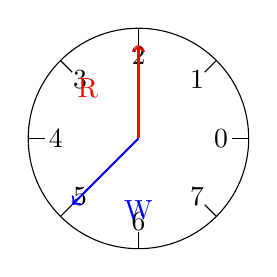
\begin{tikzpicture}[scale=0.7]
        \draw (0,0) circle (2);
        \foreach \i in {0,1,...,7} {
            \draw ({2*cos(45*\i)},{2*sin(45*\i)}) -- ({1.7*cos(45*\i)},{1.7*sin(45*\i)});
            \node at ({1.5*cos(45*\i)},{1.5*sin(45*\i)}) {\i};
        }
        \draw[->, thick, red] (0,0) -- ({1.7*cos(90)},{1.7*sin(90)});
        \node[red] at ({1.3*cos(135)},{1.3*sin(135)}) {R};
        \draw[->, thick, blue] (0,0) -- ({1.7*cos(225)},{1.7*sin(225)});
        \node[blue] at ({1.3*cos(270)},{1.3*sin(270)}) {W};
    \end{tikzpicture}
\end{columns}
\end{frame}

\begin{frame}[fragile]{Implementation Highlights}
\begin{lstlisting}[language=C++]
// Core function showing the lock-free approach
bool TryPush(const T& item) {
  const size_t current_write = write_idx_.load(std::memory_order_relaxed);
  const size_t next_write = (current_write + 1) % Size;
  
  // Check if buffer is full
  if (next_write == read_idx_.load(std::memory_order_acquire))
    return false;
  
  // Store item and update write index
  buffer_[current_write] = item;
  write_idx_.store(next_write, std::memory_order_release);
  return true;
}
\end{lstlisting}

\begin{itemize}
    \item Key features: Atomic operations, memory ordering, no locks
    \item Returns false instead of blocking when full
\end{itemize}
\end{frame}

\begin{frame}{Key Technical Features}
\begin{itemize}
    \item \textbf{Lock-free algorithm}: Using atomic variables
    \item \textbf{Memory ordering}: Careful use of memory ordering constraints
    \begin{itemize}
        \item \texttt{memory\_order\_relaxed} for initial loads
    \end{itemize}
    \item \textbf{Cache line alignment}: Preventing false sharing between indices
    \begin{itemize}
        \item Producer and consumer threads operate on different cache lines
        \item \texttt{alignas(64)} ensures indices are on separate cache lines
    \end{itemize}
    \item \textbf{Non-blocking behavior}: TryPush/TryPop never block, return boolean success
\end{itemize}
\end{frame}

\section{Testing}

\begin{frame}[fragile]{Basic Functionality Test}
\begin{itemize}
    \item Tests fundamental properties with realistic market data structures:
\begin{lstlisting}[language=C++]
struct MarketTick {
    int64_t timestamp_ns;
    std::string symbol;
    double price;
    double quantity;
    char side;  // 'B' for buy, 'S' for sell
};
\end{lstlisting}
    \item Verifies: empty buffer detection, push until full, FIFO order, etc.
\end{itemize}
\end{frame}

\begin{frame}{Market Data Pipeline Test}
\begin{itemize}
    \item Simulates realistic market data processing:
    \begin{itemize}
        \item Producer thread: generates synthetic market tick data
        \item Consumer thread: processes ticks and measures latency
    \end{itemize}
    \item Test parameters:
    \begin{itemize}
        \item 5,000 market ticks
        \item 1024-slot buffer
        \item Alternating BTC/ETH symbols
        \item Realistic price movements
    \end{itemize}
    \item Measures end-to-end latency from tick creation to processing
\end{itemize}
\end{frame}

\begin{frame}{Performance Results}
\begin{itemize}
    \item \textbf{Test machine}: Modern x86\_64 system, GCC 13.3.0, C++23, -O3
    \item \textbf{Latency measurements}:
    \begin{itemize}
        \item \textbf{Minimum}: 215 ns
        \item \textbf{Median}: 26.3 $\mu$s
        \item \textbf{99th percentile}: 3.3 ms
        \item \textbf{Maximum}: 4.6 ms
    \end{itemize}
\end{itemize}

\begin{center}
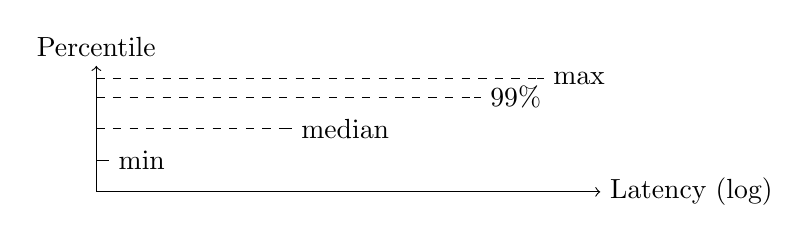
\begin{tikzpicture}[scale=0.8]
    \draw[->] (0,0) -- (8,0) node[right] {Latency (log)};
    \draw[->] (0,0) -- (0,2) node[above] {Percentile};
    
    \draw (0.1,0.5) -- (0.2,0.5) node[right] {min};
    \draw (3,1) -- (3.1,1) node[right] {median};
    \draw (6,1.5) -- (6.1,1.5) node[right] {99\%};
    \draw (7,1.8) -- (7.1,1.8) node[right] {max};
    
    \draw[dashed] (0,0.5) -- (0.1,0.5);
    \draw[dashed] (0,1) -- (3,1);
    \draw[dashed] (0,1.5) -- (6,1.5);
    \draw[dashed] (0,1.8) -- (7,1.8);
\end{tikzpicture}
\end{center}
\end{frame}

\section{Applications \& Conclusions}

\begin{frame}{Applications in Market Data Systems}
\begin{itemize}
    \item \textbf{Feed handlers}: Buffering incoming market data packets
    \item \textbf{Parsing pipeline}: Moving raw data to normalization stage
    \item \textbf{Order book updates}: Efficiently queuing price updates
    \item \textbf{Strategy components}: Communicating signals between modules
    \item \textbf{Risk checks}: Queuing pre-trade validations
    \item \textbf{Logging}: Non-blocking capture of events for later analysis
\end{itemize}
\end{frame}

\begin{frame}{Conclusions \& Next Steps}
\begin{itemize}
    \item \textbf{Achievements}:
    \begin{itemize}
        \item Created a fully lock-free, high-performance ring buffer
        \item Demonstrated functionality with real market data structures
        \item Measured sub-microsecond minimum latency
        \item Successfully processed thousands of events with predictable performance
    \end{itemize}
    \item \textbf{Potential improvements}:
    \begin{itemize}
        \item Multi-producer/multi-consumer variants
        \item Batched operations for higher throughput
        \item Memory reclamation for dynamically allocated elements
        \item Integration with hardware acceleration (FPGA, GPU)
    \end{itemize}
\end{itemize}
\end{frame}

\begin{frame}{Thank You}
\centering
\Huge{Questions?}

\vspace{1cm}
\normalsize
Our implementation is available in the project repository:\\
\texttt{src/core/ring\_buffer.h}
\end{frame}

\appendix
\section{Technical Appendix}

\begin{frame}{Atomic Operations}
\begin{itemize}
    \item \textbf{Definition}: Operations that execute completely without interference
    \item \textbf{C++ Support}: Via \texttt{std::atomic<T>} template
    \item \textbf{Key Atomic Operations}:
    \begin{itemize}
        \item \texttt{load()}: Read atomic value
        \item \texttt{store()}: Write atomic value
        \item \texttt{compare\_exchange\_*()}: Compare and swap
        \item \texttt{fetch\_add()}, \texttt{fetch\_sub()}: Atomic arithmetic
    \end{itemize}
    \item \textbf{Hardware Implementation}: Uses CPU special instructions
    \begin{itemize}
        \item x86: \texttt{LOCK} prefix, \texttt{CMPXCHG} instructions
        \item ARM: \texttt{LDREX}/\texttt{STREX} instructions
    \end{itemize}
    \item \textbf{Cost}: More expensive than regular operations but cheaper than locks
\end{itemize}
\end{frame}

\begin{frame}[fragile]{Locks and Mutexes}
\begin{columns}
\column{0.5\textwidth}
\textbf{Mutex Approach (Blocking)}
\begin{lstlisting}[language=C++]
std::mutex mtx;

void push(const T& item) {
  std::lock_guard<std::mutex> 
      lock(mtx);
  
  // Critical section
  if (buffer_full())
    wait_for_space();
    
  buffer[write_idx++] = item;
}
\end{lstlisting}

\column{0.5\textwidth}
\textbf{Issues with Mutexes}
\begin{itemize}
    \item Context switches on contention
    \item Priority inversion
    \item Kernel calls for contended locks
    \item Unpredictable latency spikes
    \item Dead/live-locks possible
\end{itemize}
\end{columns}

\textbf{Our Lock-Free Approach}: Replace mutex with atomic operations + careful algorithm design
\end{frame}

\begin{frame}{Cache Line Alignment (alignas)}
\begin{columns}
\column{0.6\textwidth}
\begin{itemize}
    \item \textbf{Cache Line}: Smallest unit of memory transferred between RAM and CPU cache
    \item Typical size: 64 bytes on modern CPUs
    \item \textbf{False Sharing Problem}:
    \begin{itemize}
        \item When two threads modify variables in same cache line
        \item Causes constant cache invalidation
        \item Significant performance impact
    \end{itemize}
    \item \textbf{Solution}: \texttt{alignas(64)}
    \begin{itemize}
        \item Ensures variables used by different threads are on different cache lines
    \end{itemize}
\end{itemize}

\column{0.4\textwidth}
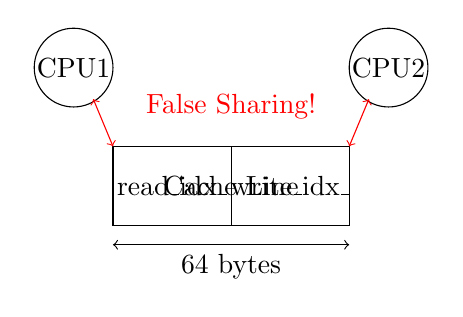
\begin{tikzpicture}[scale=0.5]
    % Cache line showing false sharing
    \draw (0,0) rectangle (6,2) node[pos=.5] {Cache Line};
    \draw (0,0) rectangle (3,2) node[pos=.5] {read\_idx\_};
    \draw (3,0) rectangle (6,2) node[pos=.5] {write\_idx\_};
    \draw[<->] (0,-0.5) -- (6,-0.5) node[below, midway] {64 bytes};
    
    % Multi-core with arrows
    \draw (-1,4) circle (1) node {CPU1};
    \draw (7,4) circle (1) node {CPU2};
    \draw[<->, red] (0,2) -- (-0.5,3.2);
    \draw[<->, red] (6,2) -- (6.5,3.2);
    \node[red] at (3,3) {False Sharing!};
\end{tikzpicture}
\end{columns}
\end{frame}

\begin{frame}[fragile]{Memory Ordering}
\begin{itemize}
    \item \textbf{Problem}: Modern CPUs reorder memory operations for performance
    \item \textbf{In Multithreaded Code}: Can cause incorrect behavior
    \item \textbf{C++ Memory Ordering Options}:
    \begin{itemize}
        \item \texttt{memory\_order\_relaxed}: No synchronization
        \item \texttt{memory\_order\_acquire}: Creates "happens-before" relationship for reads
        \item \texttt{memory\_order\_release}: Creates "happens-before" relationship for writes
        \item \texttt{memory\_order\_seq\_cst}: Full sequentially consistent ordering (expensive)
    \end{itemize}
\end{itemize}

\begin{lstlisting}[language=C++]
// In our ring buffer:
write_idx_.store(next_write, std::memory_order_release);  // Producer
//...
read_idx_.load(std::memory_order_acquire);  // Consumer
\end{lstlisting}

This creates a happens-before relationship between the buffer write and the consumer's read, ensuring the consumer sees updated data.
\end{frame}

\begin{frame}{Non-Blocking Behavior}
\begin{itemize}
    \item \textbf{Blocking API}: Waits until operation can complete
    \begin{itemize}
        \item Example: \texttt{queue.push()} might wait until space is available
        \item Unpredictable latency, potential deadlocks
    \end{itemize}
    \item \textbf{Non-Blocking API}: Returns immediately with status
    \begin{itemize}
        \item Example: \texttt{ring\_buffer.TryPush()} returns false if full
        \item Fixed, predictable latency
        \item Caller decides how to handle failure
    \end{itemize}
    \item \textbf{Benefits in Trading Systems}:
    \begin{itemize}
        \item Predictable worst-case latency
        \item No priority inversion
        \item Better behavior under pressure (fail fast vs. hang)
    \end{itemize}
    \item Our implementation is fully non-blocking
\end{itemize}
\end{frame}

\begin{frame}{Lock-Free vs. Wait-Free vs. Obstruction-Free}
\begin{itemize}
    \item \textbf{Lock-Free}: At least one thread always makes progress
    \begin{itemize}
        \item May require retries (our implementation)
        \item No deadlocks possible
    \end{itemize}
    \item \textbf{Wait-Free}: All threads make progress in bounded steps
    \begin{itemize}
        \item Strongest guarantee
        \item Most complex to implement
        \item No starvation
    \end{itemize}
    \item \textbf{Obstruction-Free}: Thread makes progress if run in isolation
    \begin{itemize}
        \item Weakest guarantee
        \item Easier to implement
    \end{itemize}
    \item \textbf{Future Work}: Consider wait-free variants for critical components
\end{itemize}
\end{frame}

\section{Deep Dive: Synchronization Costs}

\begin{frame}{Context Switches: The Hidden Cost}
\begin{columns}
\column{0.55\textwidth}
\textbf{What is a context switch?}
\begin{itemize}
    \item CPU switches execution from one thread to another
    \item Requires saving/restoring entire CPU state
    \item Triggered by:
    \begin{itemize}
        \item Thread blocking on mutex acquisition
        \item Scheduler time slice expiration
        \item Higher priority thread becoming ready
    \end{itemize}
\end{itemize}

\textbf{Costs:}
\begin{itemize}
    \item Direct: 1,000-10,000 cycles (0.5-5µs)
    \item Indirect: Cache/TLB pollution (much larger)
    \item Unpredictable scheduling delays
\end{itemize}

\column{0.45\textwidth}
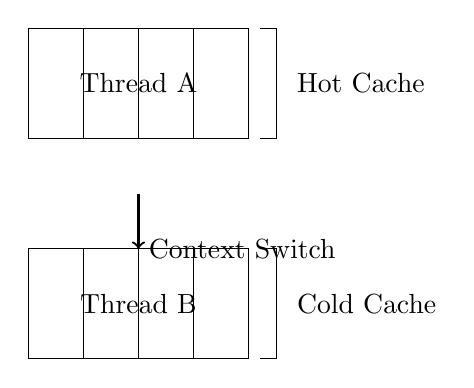
\begin{tikzpicture}[scale=0.7]
    % Before context switch
    \draw (0,4) rectangle (4,6) node[pos=.5] {Thread A};
    \draw (0,4) -- (4,4);
    \draw (1,4) -- (1,6);
    \draw (2,4) -- (2,6);
    \draw (3,4) -- (3,6);
    
    \draw[->,thick] (2,3) -- (2,2) node[right] {Context Switch};
    
    % After context switch
    \draw (0,0) rectangle (4,2) node[pos=.5] {Thread B};
    \draw (0,0) -- (4,0);
    \draw (1,0) -- (1,2);
    \draw (2,0) -- (2,2);
    \draw (3,0) -- (3,2);
    
    % Cold cache - using brackets instead of braces
    \draw (4.2,6) -- (4.5,6) -- (4.5,4) -- (4.2,4);
    \node[right] at (4.7,5) {Hot Cache};
    
    \draw (4.2,2) -- (4.5,2) -- (4.5,0) -- (4.2,0);
    \node[right] at (4.7,1) {Cold Cache};
\end{tikzpicture}
\end{columns}

\end{frame}

\begin{frame}{Context Switch Impact: Trading Example}
\begin{columns}
\column{0.6\textwidth}
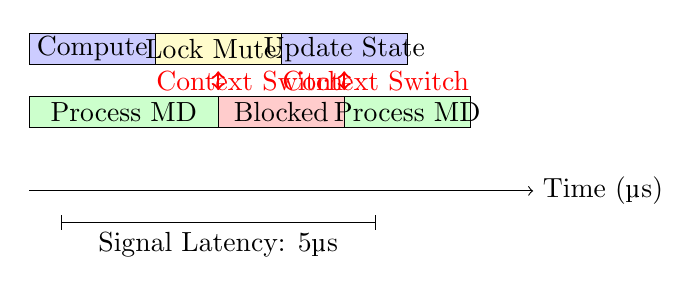
\begin{tikzpicture}[scale=0.8]
    % Timeline
    \draw[->] (0,0) -- (8,0) node[right] {Time (µs)};
    
    % Market data thread
    \draw[fill=green!20] (0,1) rectangle (3,1.5) node[pos=.5] {Process MD};
    \draw[fill=red!20] (3,1) rectangle (5,1.5) node[pos=.5] {Blocked};
    \draw[fill=green!20] (5,1) rectangle (7,1.5) node[pos=.5] {Process MD};
    
    % Strategy thread
    \draw[fill=blue!20] (0,2) rectangle (2,2.5) node[pos=.5] {Compute};
    \draw[fill=yellow!20] (2,2) rectangle (4,2.5) node[pos=.5] {Lock Mutex};
    \draw[fill=blue!20] (4,2) rectangle (6,2.5) node[pos=.5] {Update State};
    
    % Signal latency
    \draw[|-|] (0.5,-0.5) -- (5.5,-0.5) node[midway, below] {Signal Latency: 5µs};
    
    % Context switch
    \draw[<->, red, thick] (3,1.6) -- (3,1.9);
    \node[red] at (3.5,1.75) {Context Switch};
    \draw[<->, red, thick] (5,1.6) -- (5,1.9);
    \node[red] at (5.5,1.75) {Context Switch};
\end{tikzpicture}

\column{0.4\textwidth}
\textbf{Real-world impact:}
\begin{itemize}
    \item Market signal detection delayed
    \item Jittery response times
    \item Timing unpredictability
    \item Missed opportunities
\end{itemize}

\textbf{Cost in HFT:}
\begin{itemize}
    \item Each µs is critical
    \item 5µs delay can be the difference between profit and loss
    \item Context switches can add 2-10µs of latency
\end{itemize}
\end{columns}

\textbf{Lock-free advantage:} Threads never block on each other, eliminating context switches from lock contention
\end{frame}

\begin{frame}{Priority Inversion: When Priority Systems Break Down}
\begin{columns}
\column{0.55\textwidth}
\textbf{What is priority inversion?}
\begin{itemize}
    \item High-priority thread blocked by low-priority thread
    \item Low-priority thread preempted by medium-priority thread
    \item High priority thread can't run until medium priority is done
\end{itemize}

\textbf{Famous example:} Mars Pathfinder mission (1997)
\begin{itemize}
    \item Spacecraft kept rebooting on Mars
    \item High-priority task blocked on mutex
    \item Low-priority task holding mutex preempted
    \item Watchdog timer expired, causing resets
    \item Fixed by enabling priority inheritance
\end{itemize}

\column{0.45\textwidth}
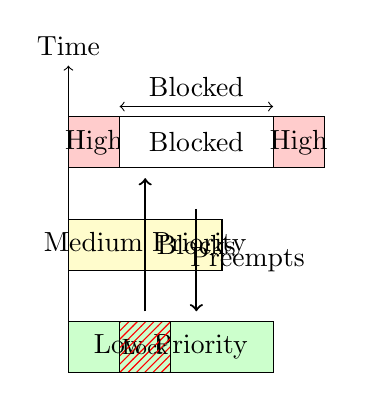
\begin{tikzpicture}[scale=0.65]
    % Timeline
    \draw[->] (0,0) -- (0,6) node[above] {Time};
    
    % Low priority
    \draw[fill=green!20] (0,0) rectangle (4,1) node[pos=.5] {Low Priority};
    \draw[pattern=north east lines, pattern color=red] (1,0) rectangle (2,1) node[pos=.5, scale=0.8] {Lock};
    
    % Medium priority
    \draw[fill=yellow!20] (0,2) rectangle (3,3) node[pos=.5] {Medium Priority};
    
    % High priority
    \draw[fill=red!20] (0,4) rectangle (1,5) node[pos=.5] {High};
    \draw[fill=white] (1,4) rectangle (4,5) node[pos=.5] {Blocked};
    \draw[fill=red!20] (4,4) rectangle (5,5) node[pos=.5] {High};
    
    % Annotations
    \draw[<->] (1,5.2) -- (4,5.2) node[midway, above] {Blocked};
    \draw[->, thick] (1.5,1.2) -- (1.5,3.8);
    \node at (2.5,2.5) {Blocks};
    \draw[->, thick] (2.5,3.2) -- (2.5,1.2);
    \node at (3.5,2.2) {Preempts};
\end{tikzpicture}
\end{columns}

\end{frame}

\begin{frame}{Priority Inversion: Market Data Example}
\textbf{Trading system scenario:}
\begin{itemize}
    \item High priority: Order execution thread (100µs SLA)
    \item Medium priority: Risk check thread
    \item Low priority: Market data processing thread
\end{itemize}

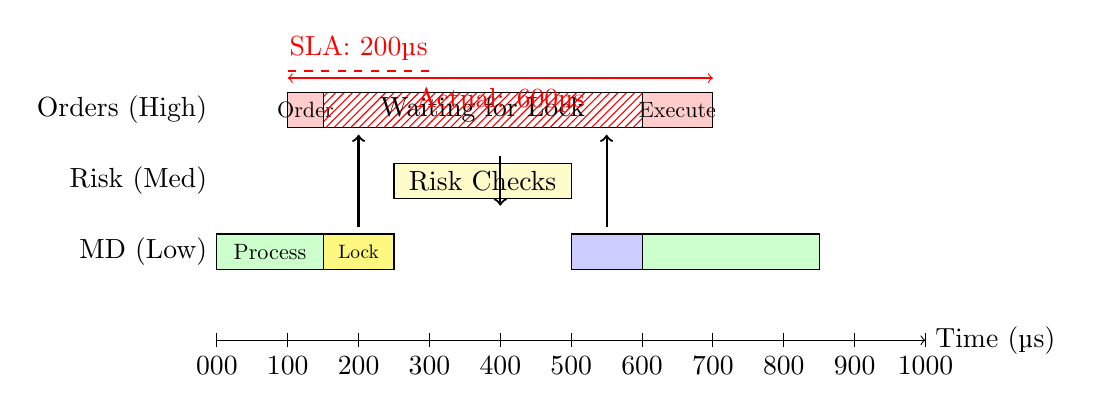
\begin{tikzpicture}[scale=0.9]
    % Timeline
    \draw[->] (0,0) -- (10,0) node[right] {Time (µs)};
    \foreach \x in {0,1,...,10} {
        \draw (\x,0.1) -- (\x,-0.1) node[below] {\x00};
    }
    
    % Market data thread (Low priority)
    \draw[fill=green!20] (0,1) rectangle (1.5,1.5) node[pos=.5, scale=0.8] {Process};
    \draw[fill=yellow!50] (1.5,1) rectangle (2.5,1.5) node[pos=.5, scale=0.7] {Lock};
    \draw[fill=blue!20] (5,1) rectangle (6,1.5);
    \draw[fill=green!20] (6,1) rectangle (8.5,1.5);
    \node[left] at (0,1.25) {MD (Low)};
    
    % Risk thread (Medium priority)
    \draw[fill=yellow!20] (2.5,2) rectangle (5,2.5) node[pos=.5] {Risk Checks};
    \node[left] at (0,2.25) {Risk (Med)};
    
    % Order thread (High priority)
    \draw[fill=red!20] (1,3) rectangle (1.5,3.5) node[pos=.5, scale=0.8] {Order};
    \draw[fill=white, pattern=north east lines, pattern color=red] (1.5,3) rectangle (6,3.5) node[pos=.5] {Waiting for Lock};
    \draw[fill=red!20] (6,3) rectangle (7,3.5) node[pos=.5, scale=0.8] {Execute};
    \node[left] at (0,3.25) {Orders (High)};
    
    % SLA
    \draw[dashed, red] (1,3.8) -- (3,3.8) node[above, midway] {SLA: 200µs};
    \draw[<->, red] (1,3.7) -- (7,3.7) node[below, midway] {Actual: 600µs};
    
    % Arrows
    \draw[->, thick] (2,1.6) -- (2,2.9);
    \draw[->, thick] (4,2.6) -- (4,1.9);
    \draw[->, thick] (5.5,1.6) -- (5.5,2.9);
\end{tikzpicture}

\textbf{Impact in trading:}
\begin{itemize}
    \item Orders delayed well beyond SLA
    \item Potential regulatory violations
    \item Financial impact from missed trades
    \item System appears "stuck" under high load
\end{itemize}

\textbf{Lock-free solution:} Eliminates shared mutex, preventing priority inversion entirely
\end{frame}

\begin{frame}[fragile]{Kernel Calls for Contended Locks}
\begin{columns}
\column{0.55\textwidth}
\textbf{What happens on mutex contention:}
\begin{enumerate}
    \item Thread attempts lock (user-space)
    \item If contended, calls \texttt{futex(FUTEX\_WAIT)} system call
    \item Control transfers to kernel
    \item Thread state changed to blocked
    \item Context switch to another thread
    \item When lock released, owner calls \texttt{futex(FUTEX\_WAKE)}
    \item Kernel performs another context switch
\end{enumerate}

\textbf{Key Issue:} User-space to kernel-space transitions
\begin{itemize}
    \item Each transition: 1,000-1,500 cycles
    \item Shared kernel data structures
    \item Privileged mode switches
    \item Scheduler involvement
\end{itemize}

\column{0.45\textwidth}
\begin{lstlisting}[language=C++, basicstyle=\tiny]
// Simplified pthread_mutex implementation
void lock_mutex(pthread_mutex_t* m) {
  // Fast path - try atomic acquisition
  if (atomic_cas(&m->locked, 0, 1) == 0)
    return; // Got the lock!
    
  // Slow path - contention
  while (1) {
    // Spin a bit first (optimistic)
    for (int i = 0; i < 100; i++) {
      if (m->locked == 0 &&
          atomic_cas(&m->locked, 0, 1) == 0)
        return;
      _mm_pause(); // CPU hint
    }
        
    // Enter kernel (expensive!)
    futex(&m->locked, FUTEX_WAIT, 1, NULL);
  }
}
\end{lstlisting}
\end{columns}
\end{frame}

\begin{frame}{Kernel Calls: Performance Impact}

\begin{columns}
\column{0.58\textwidth}
\textbf{Performance metrics on Intel i9-12900K:}
\begin{itemize}
    \item L1 cache access: 1-2 ns
    \item L3 cache access: 10-20 ns
    \item RAM access: 60-100 ns
    \item Uncontended mutex lock: 20-30 ns
    \item \textbf{Contended mutex (kernel call)}: 1,000-15,000 ns
    \item \textbf{Lock-free ringbuffer operation}: 30-50 ns
\end{itemize}

\textbf{Trading impact:}
\begin{itemize}
    \item \textbf{Tick-to-trade latency increase:} 1-15µs
    \item \textbf{Tail latencies (99th):} Can be 100x worse
    \item \textbf{Jitter:} Major increase in variability
    \item \textbf{CPU time:} Wasted on kernel transitions
\end{itemize}

\column{0.42\textwidth}
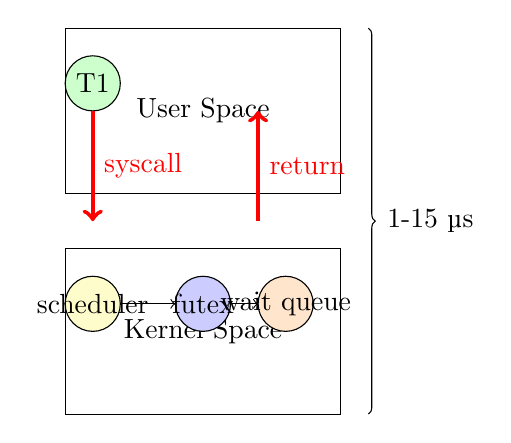
\begin{tikzpicture}[scale=0.7]
    % User vs Kernel space
    \draw (0,0) rectangle (5,3) node[pos=.5] {User Space};
    \draw (0,-4) rectangle (5,-1) node[pos=.5] {Kernel Space};
    
    % Thread in user space
    \draw[fill=green!20] (0.5,2) circle (0.5) node {T1};
    
    % Arrows
    \draw[->, ultra thick, red] (0.5,1.5) -- (0.5,-0.5) node[midway, right] {syscall};
    \draw[->, ultra thick, red] (3.5,-0.5) -- (3.5,1.5) node[midway, right] {return};
    
    % Kernel components
    \draw[fill=yellow!20] (0.5,-2) circle (0.5) node {scheduler};
    \draw[fill=blue!20] (2.5,-2) circle (0.5) node {futex};
    \draw[fill=orange!20] (4,-2) circle (0.5) node {wait queue};
    
    % Connecting arrows in kernel
    \draw[->] (1,-2) -- (2,-2);
    \draw[->] (3,-2) -- (3.5,-2);
    
    % Latency impact
    \draw[decorate, decoration={brace}] (5.5,3) -- (5.5,-4) node[midway, right] {~1-15 µs};
\end{tikzpicture}
\end{columns}

\textbf{Lock-free advantage:} Operations stay entirely in user space, avoiding kernel transitions completely
\end{frame}

\begin{frame}{Comparison: Lock-Based vs. Lock-Free Architecture}
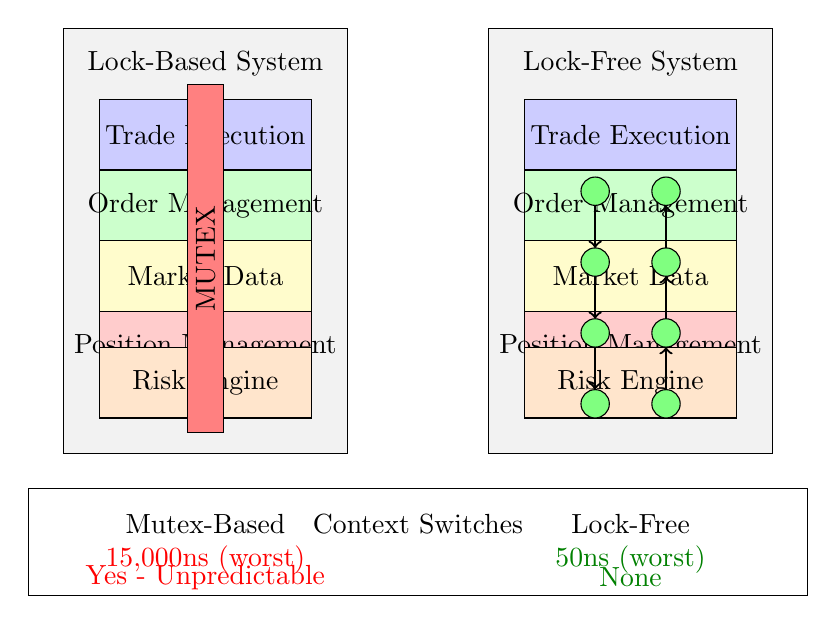
\begin{tikzpicture}[scale=0.9]
    % Lock-based system
    \draw[fill=gray!10] (0,0) rectangle (4,6);
    \node at (2,5.5) {Lock-Based System};
    
    % Components
    \draw[fill=blue!20] (0.5,4) rectangle (3.5,5) node[pos=.5] {Trade Execution};
    \draw[fill=green!20] (0.5,3) rectangle (3.5,4) node[pos=.5] {Order Management};
    \draw[fill=yellow!20] (0.5,2) rectangle (3.5,3) node[pos=.5] {Market Data};
    \draw[fill=red!20] (0.5,1) rectangle (3.5,2) node[pos=.5] {Position Management};
    \draw[fill=orange!20] (0.5,0.5) rectangle (3.5,1.5) node[pos=.5] {Risk Engine};
    
    % Locks
    \draw[fill=red!50] (1.75,0.3) rectangle (2.25,5.2) node[pos=.5, rotate=90] {MUTEX};
    
    % Lock-free system
    \draw[fill=gray!10] (6,0) rectangle (10,6);
    \node at (8,5.5) {Lock-Free System};
    
    % Components
    \draw[fill=blue!20] (6.5,4) rectangle (9.5,5) node[pos=.5] {Trade Execution};
    \draw[fill=green!20] (6.5,3) rectangle (9.5,4) node[pos=.5] {Order Management};
    \draw[fill=yellow!20] (6.5,2) rectangle (9.5,3) node[pos=.5] {Market Data};
    \draw[fill=red!20] (6.5,1) rectangle (9.5,2) node[pos=.5] {Position Management};
    \draw[fill=orange!20] (6.5,0.5) rectangle (9.5,1.5) node[pos=.5] {Risk Engine};
    
    % Ring buffers
    \draw[fill=green!50] (7.5,3.7) circle (0.2);
    \draw[fill=green!50] (8.5,3.7) circle (0.2);
    \draw[fill=green!50] (7.5,2.7) circle (0.2);
    \draw[fill=green!50] (8.5,2.7) circle (0.2);
    \draw[fill=green!50] (7.5,1.7) circle (0.2);
    \draw[fill=green!50] (8.5,1.7) circle (0.2);
    \draw[fill=green!50] (7.5,0.7) circle (0.2);
    \draw[fill=green!50] (8.5,0.7) circle (0.2);
    
    % Arrows
    \draw[->, thick] (7.5,3.5) -- (7.5,2.9);
    \draw[->, thick] (8.5,2.9) -- (8.5,3.5);
    \draw[->, thick] (7.5,2.5) -- (7.5,1.9);
    \draw[->, thick] (8.5,1.9) -- (8.5,2.5);
    \draw[->, thick] (7.5,1.5) -- (7.5,0.9);
    \draw[->, thick] (8.5,0.9) -- (8.5,1.5);
    
    % Comparison metrics
    \draw (-0.5,-0.5) rectangle (10.5,-2);
    \node at (2,-1) {Mutex-Based};
    \node at (8,-1) {Lock-Free};
    \node[red] at (2,-1.5) {15,000ns (worst)};
    \node[green!50!black] at (8,-1.5) {50ns (worst)};
    \node at (5,-1) {Context Switches};
    \node[red] at (2,-1.75) {Yes - Unpredictable};
    \node[green!50!black] at (8,-1.75) {None};
\end{tikzpicture}
\end{frame}

% ====================================================================
% SECTION: Ring Buffer Optimization - False Sharing & Memory Alignment
% ====================================================================

\section{Ring Buffer Optimization}

% Slide: The Performance Killer - False Sharing
\begin{frame}
  \frametitle{The Performance Killer: False Sharing}
  
  \begin{itemize}
    \item \textbf{False sharing}: Multiple threads accessing \textit{different} data that happens to be on the \textit{same} cache line
    \item Our benchmark showed \textbf{8.7x performance penalty} when counters shared a cache line
    \item 59\% more cache misses in unaligned version
    \item Critical for ring buffer implementation where producer and consumer often run on different cores
  \end{itemize}
  
  \begin{alertblock}{Definition}
    False sharing occurs when two threads modify different variables that happen to be on the same cache line, causing unnecessary cache invalidations
  \end{alertblock}
\end{frame}

% Slide: Cache Lines Explained
\begin{frame}
  \frametitle{Cache Lines Explained}
  
  \begin{itemize}
    \item Modern CPUs load memory in fixed-size blocks called \textbf{cache lines} (typically 64 bytes)
    \item If one core modifies \textit{any byte} in a cache line, other cores must reload the \textit{entire line}
    \item Ring buffer hot spots:
    \begin{itemize}
      \item Read index (consumer)
      \item Write index (producer)
      \item If these share a cache line → major performance penalty
    \end{itemize}
  \end{itemize}
  
  \begin{alertblock}{Key Insight}
    Sharing a cache line between threads is like sharing a notepad - even if you're writing on different pages!
  \end{alertblock}
\end{frame}

% Slide: Scaling Problems with False Sharing
\begin{frame}
  \frametitle{Scaling Problems with False Sharing}
  
  \begin{center}
    \begin{tabular}{|l|r|r|r|}
      \hline
      \textbf{Thread Count} & \textbf{Unaligned Time} & \textbf{Aligned Time} & \textbf{Slowdown} \\
      \hline
      4 threads & 3798 ms & 436 ms & 8.7x \\
      8 threads & 11285 ms & 4225 ms & 2.7x \\
      16 threads & 14310 ms & 5007 ms & 2.9x \\
      24 threads & 15607 ms & 4497 ms & 3.5x \\
      \hline
    \end{tabular}
  \end{center}
  
  \begin{itemize}
    \item Performance penalty grows with core count
    \item A properly aligned ring buffer will scale much better
    \item Dramatic difference in cache misses (30\% fewer in aligned version)
  \end{itemize}
\end{frame}

% Slide: Ring Buffer Optimized Design
\begin{frame}[fragile]
  \frametitle{Ring Buffer Optimized Design}
  
  \begin{columns}
    \begin{column}{0.55\textwidth}
      \begin{lstlisting}[language=C++]
struct alignas(64) RingBuffer {
    // Producer variables
    std::atomic<size_t> write_idx{0};
    char pad1[64 - sizeof(std::atomic<size_t>)];
    
    // Consumer variables
    std::atomic<size_t> read_idx{0};
    char pad2[64 - sizeof(std::atomic<size_t>)];
    
    // Buffer contents
    T data[BUFFER_SIZE];
};
      \end{lstlisting}
    \end{column}
    
    \begin{column}{0.45\textwidth}
      \begin{itemize}
        \item Keep read/write indices on separate cache lines
        \item Padding ensures no false sharing
        \item 30\% fewer cache misses
        \item Up to 8.7x faster operation
        \item Small memory trade-off for huge performance gain
      \end{itemize}
    \end{column}
  \end{columns}
\end{frame}

% Slide: Memory Ordering Matters Too
\begin{frame}
  \frametitle{Memory Ordering Matters Too}
  
  \begin{itemize}
    \item False sharing isn't the only concern
    \item Proper memory ordering ensures correctness:
    \begin{itemize}
      \item \texttt{std::memory\_order\_relaxed}: Fastest but may reorder operations
      \item \texttt{std::memory\_order\_acquire}/\texttt{release}: Ensures proper happens-before relationships
      \item Ring buffer typically needs acquire-release semantics for correctness
    \end{itemize}
  \end{itemize}
  
  \begin{exampleblock}{Relaxed vs. Acquire-Release}
    Our tests showed that relaxed ordering might output "42" in all cases, but it's \\
    not guaranteed. Acquire-release provides the necessary synchronization guarantees.
  \end{exampleblock}
\end{frame}

% Slide: Key Takeaways
\begin{frame}
  \frametitle{Key Takeaways for Ring Buffer Implementation}
  
  \begin{enumerate}
    \item \textbf{Align critical data} to cache line boundaries (typically 64 bytes)
    \item \textbf{Separate read/write indices} onto different cache lines
    \item \textbf{Use appropriate memory ordering} for both performance and correctness
    \item \textbf{Benchmark with multiple threads} to verify scaling
  \end{enumerate}
  
  \begin{alertblock}{Performance vs. Space Trade-off}
    Cost: Slightly higher memory usage (256 bytes vs 32 bytes in our example)\\
    Benefit: Up to 8.7x performance improvement under contention
  \end{alertblock}
  
  \begin{center}
    \large{For low-latency systems, cache alignment is not optional!}
  \end{center}
\end{frame}

\end{document}